\documentclass[a4paper,11pt]{article}
\usepackage[utf8]{inputenc}
\usepackage{graphicx}
\usepackage{amsfonts}
\usepackage[normalem]{ulem}
\usepackage{hyperref}
\begin{document}


\section{CÁLCULOS TEÓRICOS}
Fuente de alimentación: 9 Voltios

	\begin{figure}[h]
		\caption{TRANSMISOR INFRAROJO}
		\centering
		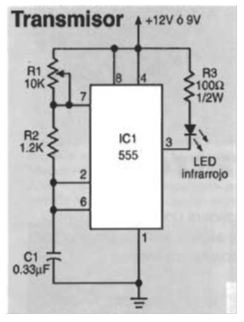
\includegraphics[width=0.4\linewidth]{./19}
	\end{figure}
	
	\begin{figure}[h]
		\centering
		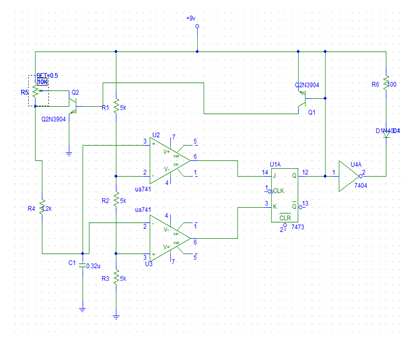
\includegraphics[width=0.7\linewidth]{./20}
	\end{figure}	
\newpage
$$V_a = \frac{2}{3}V_{cc}V_b = \frac{1}{3}V_{cc}$$
$$V_a = 6v \ \ \ V_b = 3v$$
$$V_c = 0v$$
$\begin{array}{lcl}
U_1: & V_c = 0v & S=0 \\
	& V_a = 6v &
\end{array}$
$$\rightarrow Q = 0 \ V_0= +V_{cc} \ \rightarrow LED \ off$$

$\begin{array}{lcl}
U_2: & V_c = 0v & R = 1\\
	& V_a = 3v &
\end{array}$

$$V_c = 3v$$
$\begin{array}{lcl}
U_1: & V_c = 3v & S=0 \\
	& V_a = 6v &
\end{array}$
$$\rightarrow Q = Mantiene \ V_0= +V_{cc} \ \rightarrow LED \ off$$
$$U_2 \ Cambia \ de \ estado \ R=0$$

$$V_c = 6v \rightarrow U_1: \ Cambia \ de \ estado S = 1d$$
$$\rightarrow Q=1 \ V_0= +V_{cc} \rightarrow LED on$$
$\begin{array}{lcl}
U_2: & V_c = 6v & R = 0 \ y \ empieza \ la \ oscilaci\acute{o}n \\
	& V_a = 3v & 
\end{array}$

\textbf{Carga del capacitor}

Pot. Posición Mínima R = 10k
$$tcarga = RC ln(\frac{V_{cc}-0}{V_{cc}-3})$$
$$tcarga = 1.498ms = T_a$$

Pot. Posición Máxima R = 0
$$tcarga = RC ln(\frac{V_{cc}-0}{V_{cc}-3})$$
$$tcarga = 0.16 ms = T_a$$

Pot. Posición Mínima R = 10k
$$f = \frac{1}{T_a + T_b} = 2.304KHz$$

\begin{figure}[h]
	\centering
	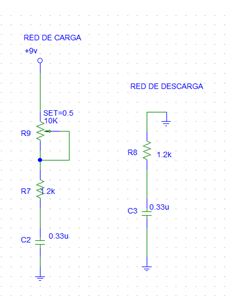
\includegraphics[width=0.7\linewidth]{./21a}
\end{figure}

Pot. Posición Mínima R = 10k
\textbf{Descarga del capacitor}
$$f= \frac{1}{T_a + T_b} = 0.564 KHz$$
$$0.564KHz<f<2.304 KHz$$
R = 1.2k
$$tdescarga = RCln(\frac{V_{cc} - 0}{V_{cc} - 3})$$
$$tcarga = 0.274 ms = T_b$$

\begin{itemize}
\item Al emisor infrarrojo lo alimenta una onda cuadrada con una frecuencia igual a la fijada en el PLL del circuito receptor. Esta frecuencia debe estar en el rango de [0.564KHz-2.304KHz]
\item La resistencia en serie con el transmisor IR limita la corriente a través del mismo, pero no reduce mucho el voltaje que lo alimenta, podemos considerar que la onda cuadrada que lo alimentara tendrá una amplitud de aprox. 9v
\end{itemize}

\newpage
\textbf{Receptor infrarrojo}

Se asume que la señal que recibe el receptor es la misma onda que envió el receptor es decir, con la misma amplitud y frecuencia. Aunque esto tiene una limitante la cual está dada por la distancia de separación entre ambos circuitos, transmisor y receptor.
Seguidamente la señal recibida pasa por un seguidor de voltaje para impedir que se filtre ruido y que exista acople de impedancias que puedan reducir el voltaje de la señal. Luego entra a un Opamp LM358 configurado como comparador en el cual compara la señal variable en el tiempo con un voltaje de referencia igual a: +9v

\begin{figure}[h]
	\centering
	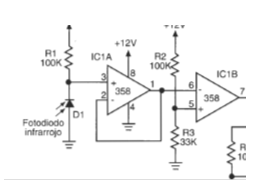
\includegraphics[width=0.7\linewidth]{./22a}
\end{figure}

$$V^- = se\tilde{n}al \ recibida \ por \ el \ fototransistor$$
$$V^+ = 9x \frac{(33)}{(100+33)} = 2.33 V \rightarrow \ Voltaje \ de \ comparaci\acute{o}n.$$

Ambas señales se compararan y dependiendo de la comparación a la salida del 358 tendremos 0v o 9v. Como una de las señales es una onda cuadrada entonces a la salida tendremos también una onda cuadrada pero invertida porque la señal variable entra por el pin (-). Luego esta señal es la entrada de un PLL.

\newpage
\textbf{PLL (enganche de fase)}

\begin{figure}[h]
	\centering
	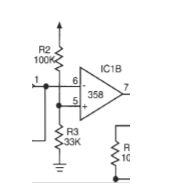
\includegraphics[width=0.3\linewidth]{./23}
	\caption{Receptor}
\end{figure}

La frecuencia prefijada en el PLL está fijada por:
$$f_0= \frac{1}{((1.1)(R4)(C1))}$$
$$f_0= \frac{1}{((1.1)(10k)(0.1u))} = 0.909KHz$$

Y el ancho de banda del integrado esta dado por:
$$BW = 1070 \sqrt{\frac{v_i}{f_0xC_3}} = porcentaje \ de \ f_0, \ C_3 \ en \mu f $$
$$V_i = 9V_p \ y \ C_3=1\mu f$$
$$BW = 11.22 \%$$

\textbf{Cuando el lazo quede enganchado en fase la salida en el pin 8 es un alto 9v.}
La señal en el pin 8 del PLL nos permitirá controlar el relay. Si la salida es un alto, +Vcc, entonces el relay no conmutara porque el transistor usado para su control estaría en corte. Pero si la salida es un bajo entonces con esto lograremos que el transistor PNP se sature y haga circular  una corriente a través de la bobina del relay y lo haga conmutar.
Al conmutar el relé activara el transmisor RF y este a su vez enviara una señal al receptor RF para que la procese y active un circuito de alarma.


La señal que se procesa es una señal digital ya que el receptor infrarrojo es un integrado que permite ser alimentado con máximo 5v. Para ello usamos un regulador de voltaje LM7805 para obtener la salida deseada.

\newpage
\textbf{Simulaciones}

\begin{figure}[h]
	\caption{EMISOR RECEPTOR-INFRARROJO}
	\centering
	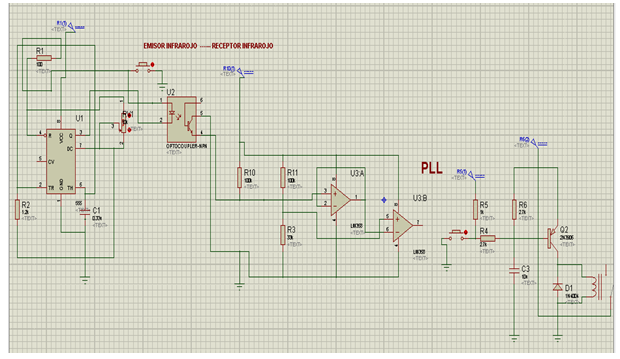
\includegraphics[width=1.1\linewidth]{./25}
\end{figure}

\begin{figure}[h]
	\caption{CUANDO SE TRANSMITE (sin colocar obstáculo) 
	Señal de voltaje en el cátodo del transmisor  infrarrojo (salida del LM555)
	}
	\centering
	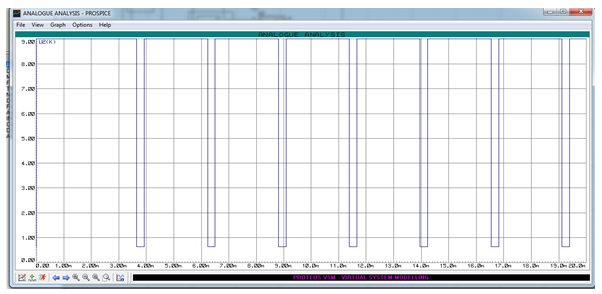
\includegraphics[width=0.8\linewidth]{./26}
\end{figure}

Esta señal es la que polariza el emisor infrarrojo y la cual será transmitida al circuito receptor mientras no se coloque un obstáculo entre ambos. La señal es una onda cuadrada con amplitud igual a la alimentación del circuito (+9v)  y una frecuencia de aproximadamente 384.615 Hz

\newpage
\begin{figure}[h]
	\caption{Señal de voltaje en el receptor infrarrojo
	}
	\centering
	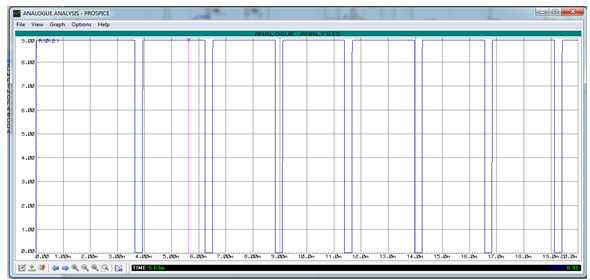
\includegraphics[width=0.7\linewidth]{./27}
\end{figure}

Las gráficas de voltaje es similar a la que se transmite, debido a que la onda no es de muy alta frecuencia entonces tendrá una limitante la cual está dada por la separación del emisor y receptor es decir habrá un instante en el cual él la onda enviada transmitida se atenuara por completo y el receptor no detectara nada.

\begin{figure}[h]
	\caption{Señal de voltaje de entrada en el PLL analógico
	}
	\centering
	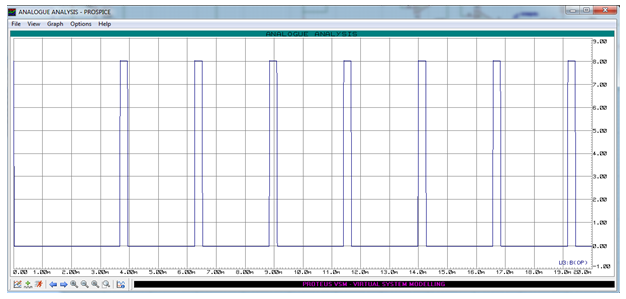
\includegraphics[width=0.7\linewidth]{./28}
\end{figure}


\textbf{CUANDO NO SE TRANSMITE (presencia de un obstáculo)} \\
Cuando colocamos nuestra mano entre el transmisor y receptor infrarrojo la señal en el receptor es nula.

\textbf{Circuito de Radiofrecuencia}
Los módulos usados para la transmisión RF son:
\begin{itemize}
	\item	Decodificador HT12E
	\item 	Módulo TPE434A
	\item 	Decodificador HT12D
\end{itemize}

\newpage
Se usa modulación ASK

\begin{figure}[h]
	\centering
	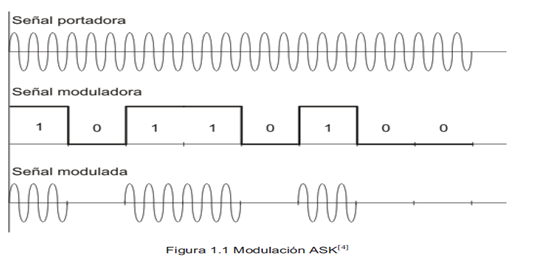
\includegraphics[width=0.7\linewidth]{./29}
\end{figure}


\begin{figure}[h]
	\centering
	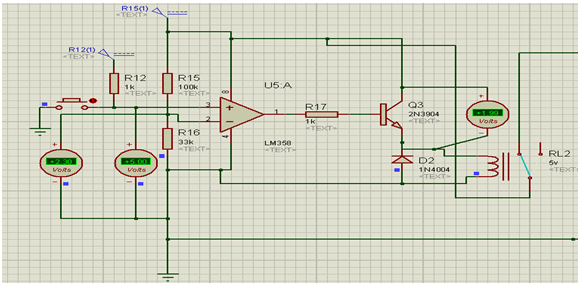
\includegraphics[width=0.7\linewidth]{./30}
\end{figure}

En esta etapa se recibe un alto proveniente de la puerta OR utilizada a la salida del decoder HT12D el cual va conectado al pin 3 del LM358 y va a ser comparado con un voltaje establecido entre un divisor de tensión que va conectado al pin2. Los voltajes comparados son pin 3 (5V) y en el pin 2 (2.3V) lo cual provoca que la salida del LM358 en el pin 1 sea +Vcc (9V en este caso) con lo cual logramos saturar el transistor Q3 y switchear el relé que nos activa el circuito de la alarma.

\newpage
\begin{figure}[h]
	\caption{CIRCUITO RECEPTOR RF - ALARMA}
	\centering
	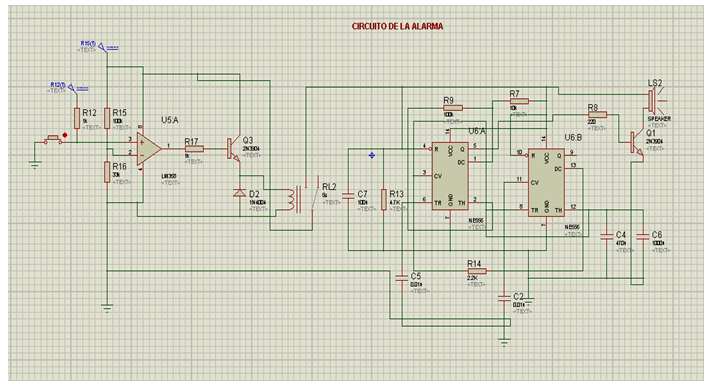
\includegraphics[width=0.8\linewidth]{./31}
\end{figure}


\begin{figure}[h]
	\caption{Señales a la salida del integrado LM556 y colector del transistor que alimenta al parlante}
	\centering
	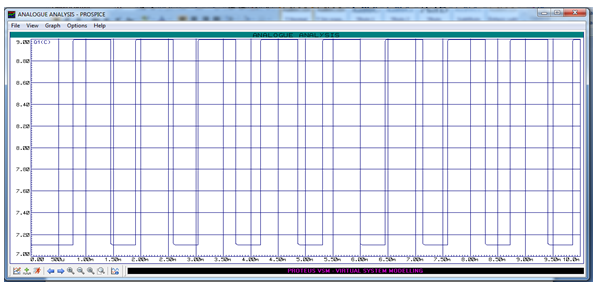
\includegraphics[width=0.7\linewidth]{./32}
\end{figure}

La señal de amarillo representa la salida del temporizador LM556 la cual va conectada a la base de un transistor cuyo voltaje de colector representado por la grafica de color azul alimenta a la alarma empleada en el proyecto. 
\newpage

\begin{figure}[h]
	\caption{Corriente a través del parlante de 8 ohms}
	\centering
	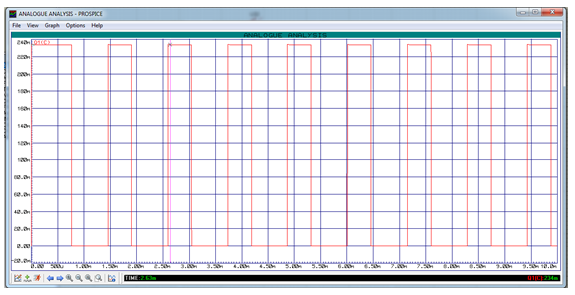
\includegraphics[width=0.7\linewidth]{./33}
\end{figure}

Esta corriente variable es la que provoca el sonido del parlante excitando la bobina móvil en el interior del mismo y provocando una onda mecánica que está dentro del rango de frecuencias que el oído humano puede detectar (20Hz – 20KHz)

\newpage
\section{Conclusiones}
\begin{itemize}
	\item Se pudo comprobar que la onda de luz natural al poseer una frecuencia mayor a la frecuencia en la cual se transmite la ráfaga de pulsos del emisor infrarrojo, esto hace que interfiera en el funcionamiento de esta etapa del proyecto, por lo que se recomienda utilizar un fototransistor infrarrojo como los que se utilizan en los televisores que lo que hacen es demodular la frecuencia con la portadora a la cual se transmite la señal infrarroja.
	\item Se logró la implementación de una etapa del circuito el cual nos permitiera poder acoplar el circuito de la alarma que fue la parte que más se nos dificulto en el proyecto, esto debido a que al utilizar una de las salidas del decoder HT12D para acoplar la alarma nos dimos cuenta que la corriente de salida de ese pin era aproximadamente cero, es decir muy bajo tanto así que no era suficiente ni para activar un buzzer, con lo que tuvimos que investigar hallando la solución al problema en el cual hubo que utilizar una puerta lógica OR entre esta salida y el pin de Valid Transmission con lo cual obtuvimos una corriente considerable con la cual polarizar un transistor para poder switchear un relé el cual nos energizara el circuito de la alarma.
	\item Se comprobó el funcionamiento del circuito mediante la realización del mismo y la comparación con los datos obtenidos en la simulación.
	\item Gracias al análisis experimental, práctico y uso de conocimientos adquiridos en los cursos de electrónica vistos en la carrera se pudo solucionar el switcheo innecesario del relé ubicado en el circuito del receptor infrarrojo que hacia trabajar de manera errónea al proyecto en totalidad debido que al energizar el proyecto y sin que exista una interrupción entre la comunicación entre los infrarrojos este se switcheaba poniendo en marcha el funcionamiento del proyecto lo que se logró solucionar quitando un capacitor ubicado ente la salida del integrado LM567 y la base del transistor BJT que permitía switchear el relé.
\end{itemize}

\section{Recomendaciones}
\begin{itemize}
	\item Verificar el cableado del circuito en el protoboard para que no queden cables al aire o existan cortocircuitos.
	\item Procurar tener todos los elementos a la mano antes de empezar el cableado.
	\item Disponer de un simulador completo en el cual se encuentren todos los componentes que haya en el circuito para lograr una correcta simulación del mismo.
	\item Verificar todo el cableado antes de energizar el circuito ante la presencia de un corto para no dañar ni quemar ningún integrado.
	\item Utilizar el tamaño adecuado para las pistas y los pines de los integrados en la elaboración del PCB para que de esta manera al momento de soldar no se levante ninguna pista.
	\item Soldar de manera uniforme y con un cautín en buen estado para así no unir pistas las cuales no deberían de ir puenteadas.
	\item Utilizar diluyente o algún limpiador de contactos eléctricos para limpiar la placa de los residuos que quedan en ella una vez terminado de soldarlas.
	\item Utilizar los paquetes adecuados de cada elemento en la elaboración de la placa para así no tener muchos cables en el aire.
\end{itemize}

\section{Bibliografía}
\begin{itemize}
	\item CEKIT 34 proyectos de electrónica PDF.
	\item \url{http://robots-argentina.com.ar/Prueba_RFLink.htm} (Comunicación-Radiofrecuencia. Prueba de un enlace de Radiofrecuencia por Eduardo J. Carletti)
	\item \url{http://robots-argentina.com.ar/Prueba_RFLink.htm}
	\item \url{http://es.scribd.com/doc/3678453/SENSOR-INFRARROJO-Teoria-y-practica}
	\item \url{http://www.uv.es/marinjl/electro/555.htm}
	\item \url{http://www.x-robotics.com/hardware.htm}
\end{itemize}
\end{document}